
SYCL程序可以是单个源文件,意味着同一个源码单元(通常是源文件及其头文件)既包含定义要在SYCL设备上执行的计算内核的代码,也包含调度这些内核执行的主机代码。图2-1显示了这两个代码路径,图2-2给出了标有主机和设备代码区域的应用示例。\par

将设备代码和主机代码合并到单个源文件(或源码单元)可以更容易地理解和维护异构应用程序。这种组合还提供了语言类型的安全性,编译器可以对代码进行更多的优化。\par

\hspace*{\fill} \\ %插入空行
图2-1 单个源文件代码包含主机代码(在CPU上运行)和设备代码(在SYCL设备上运行)
\begin{center}
	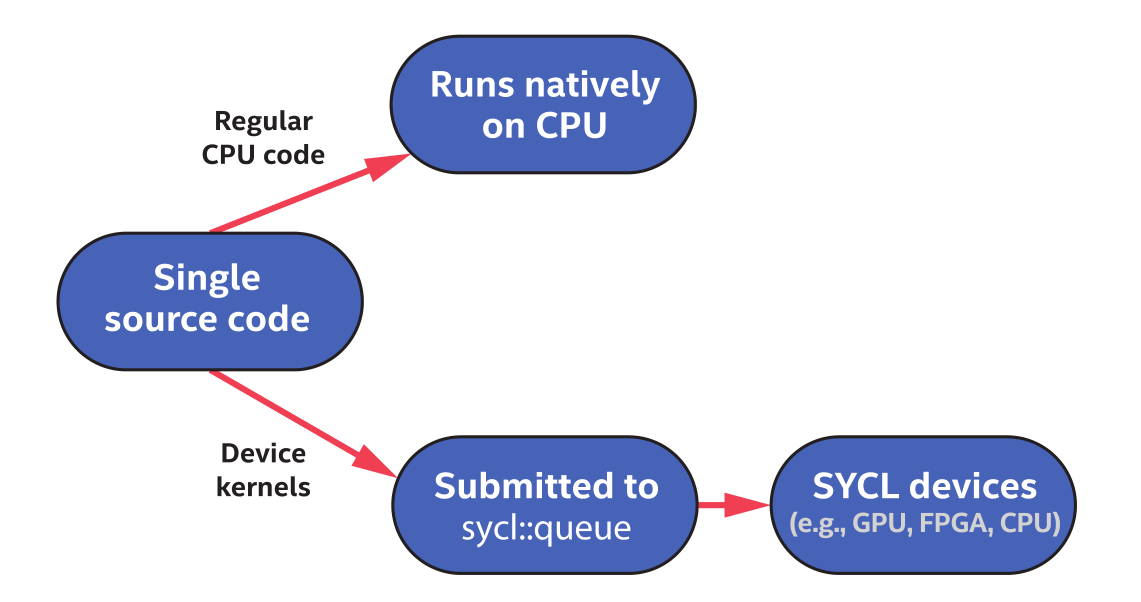
\includegraphics[width=0.8\textwidth]{content/chapter-2/images/2}
\end{center}

\hspace*{\fill} \\ %插入空行
图2-2 简单的SYCL程序
\begin{center}
	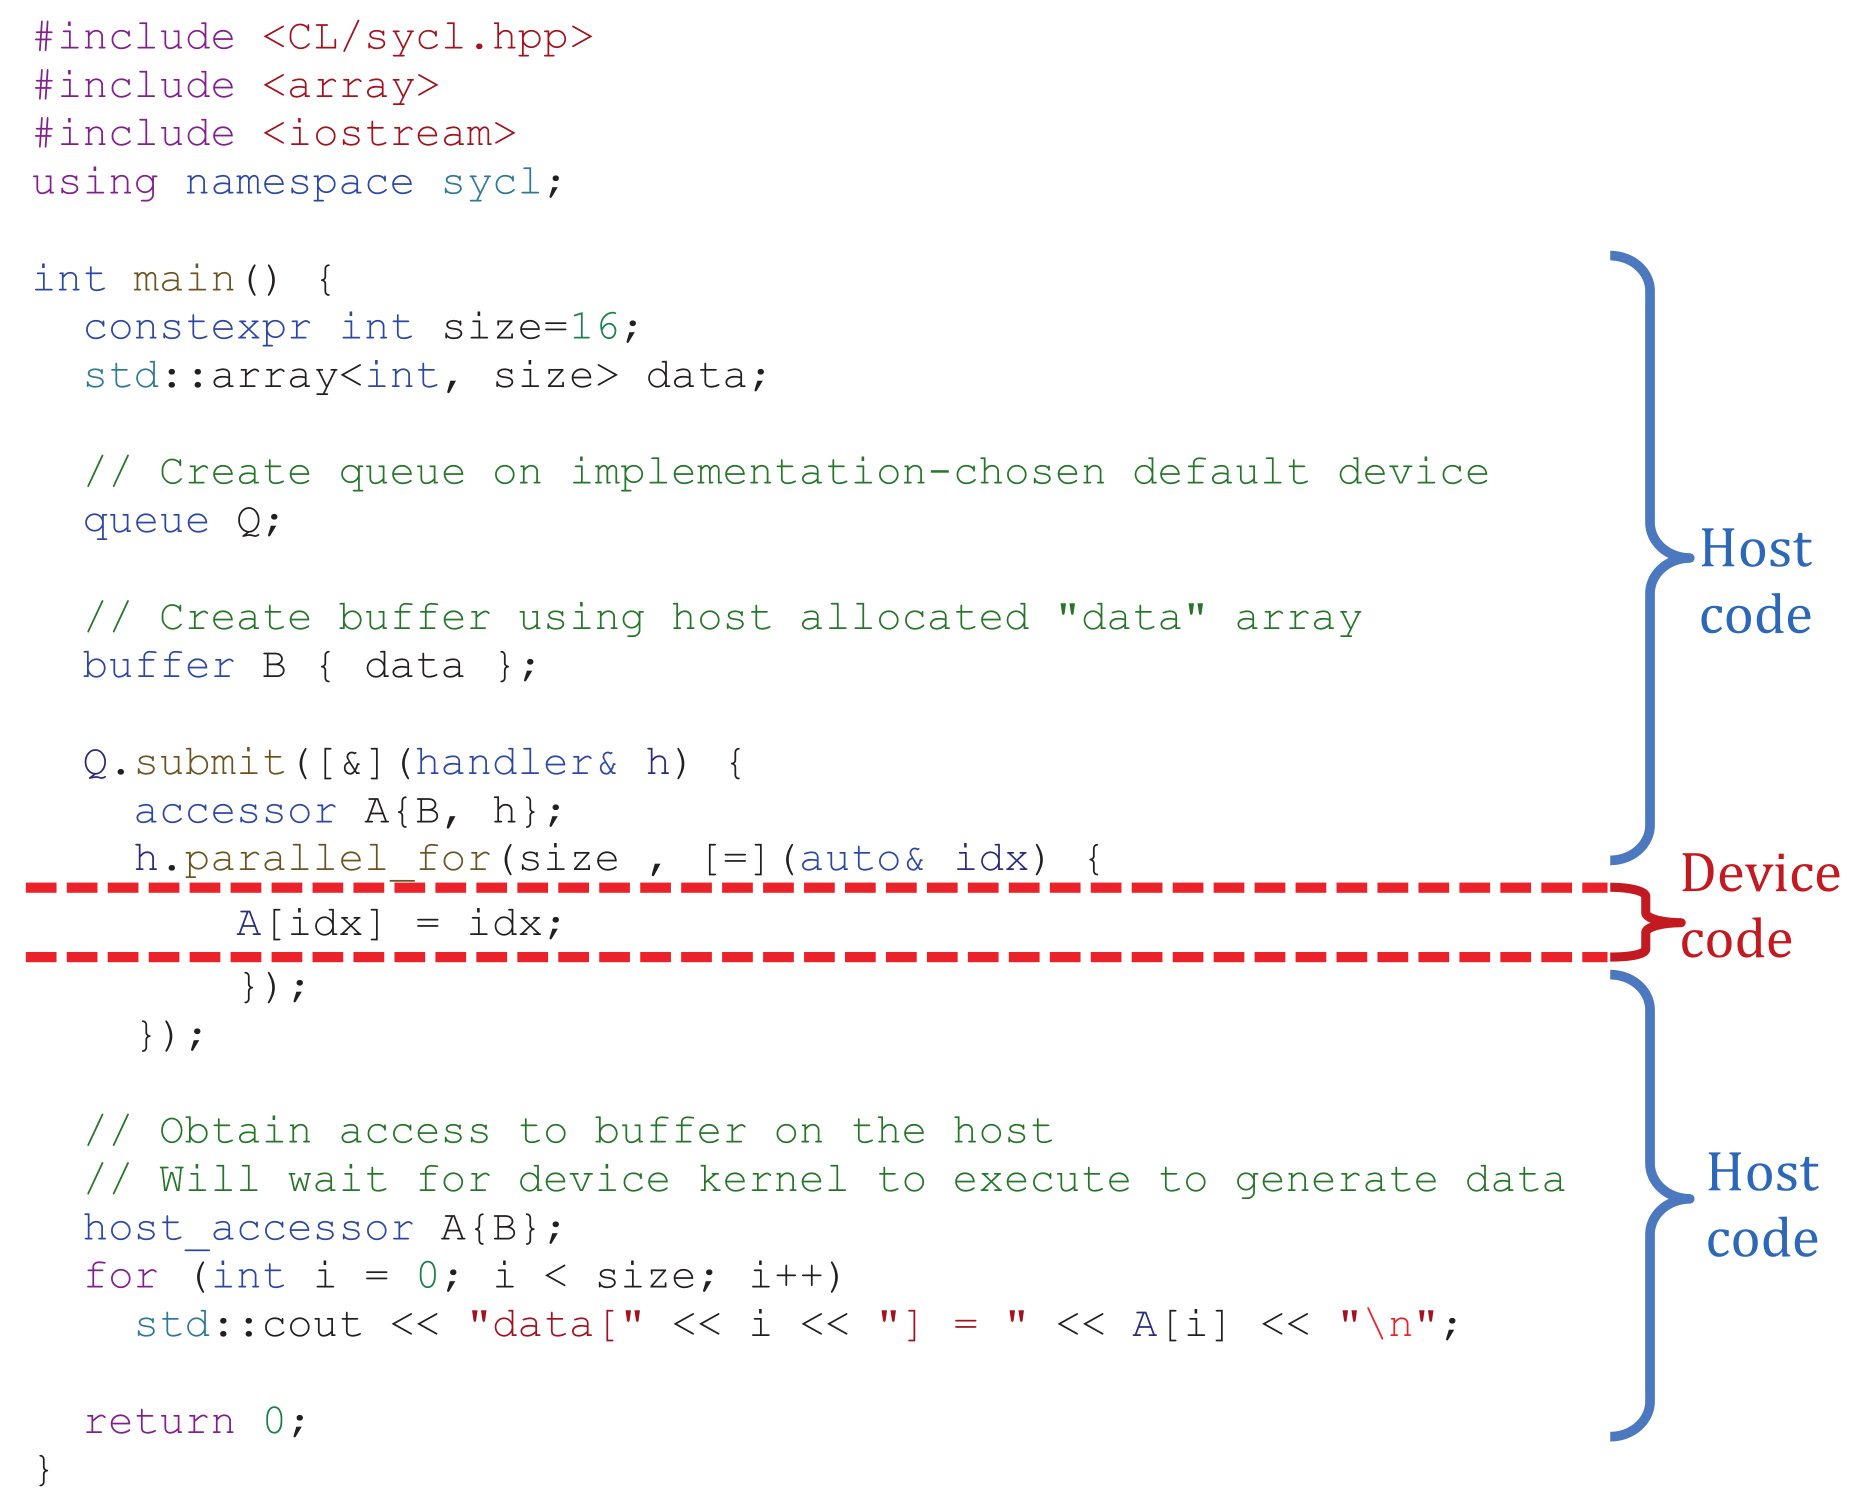
\includegraphics[width=1.\textwidth]{content/chapter-2/images/3}
\end{center}

\hspace*{\fill} \par %插入空行
\textbf{主机端代码}

应用程序包含C++主机代码,由操作系统启动CPU执行应用。主机端代码是应用程序的主要部分,它定义和控制对可用设备的工作分配,也是定义运行时数据和依赖项的接口。\par

主机端代码是用特定于SYCL的构造和类扩展的C++标准,这些构造和类设计可实现为C++库。这使得主机端代码(只要C++允许)变得更容易,并且可以简化与构建系统的集成。\par

\begin{tcolorbox}[colback=red!5!white,colframe=red!75!black]
SYCL应用是用扩充的C++标准,可以实现为C++库。\\
通过“理解”这些库,SYCL编译器可以为程序提供更高的性能。
\end{tcolorbox}

应用程序中的主机端代码会协调设备端数据移动和计算,也可以执行计算密集型工作,并可以使用任何C++的库。\par

\hspace*{\fill} \par %插入空行
\textbf{设备端代码}

设备对应于加速器或处理器,在概念上独立于执行主机代码的CPU。主机处理器也可以作为一个设备,如本章后面所述,但是主机处理器和设备应该是逻辑上相互独立的。主机处理器运行本机C++代码,而设备运行设备端代码。\par

队列是一种将工作提交给设备执行的机制。设备代码有三个重要的属性:\par

\begin{itemize}
	\item \textbf{主机端代码会异步执行。} 主机程序向设备提交设备代码,运行库只在满足所有的执行依赖关系时才跟踪和启动,并且主机程序在提交在设备上启动之前执行。提供一个属性,即设备上的执行与主机程序异步,除非显式地将两者结合在一起。
	\item \textbf{对设备代码有限制}在加速设备上编译和实现性能。例如,设备代码不支持动态内存分配和运行时类型信息(RTTI),因为它们会导致许多加速器的性能下降。设备代码限制的小集合将在第10章中详细介绍。
	\item \textbf{SYCL定义的一些函数和查询只能在设备代码中使用},例如:工作项标识符查询,允许设备代码的执行实例查询其在数据范围内的位置(在第4章中描述)。
\end{itemize}

通常,我们将包括提交在内的工作称为操作。在第3章中,我们将学习执行设备代码,还包括内存移动命令。本章中,我们关注的是操作的设备代码方面,所以将在大部分时间里提及设备端代码。\par


